\section{Output functions}


\subsection{xlpIO}

\begin{xlpfunctitle}{xlpIO}

\begin{xlpfunc}{Parameters}
\begin{tabular}{p{3.5cm}cl}
\textbf{lines}& : & number of lines \\
\textbf{trigger}& : & trigger 
\end{tabular}
\end{xlpfunc}


\begin{xlpfunc}{Returns}
A cell matrix of dimension (lines, 3)
\end{xlpfunc}

\begin{xlpfunc}{Description}
\xlp has a circular buffer of 2048 lines storing the standart ouput messages coming from python or c++ (stdout, stderr, std::cout, std::cerr). This function allows to retrieve a view of the last messages. The argument lines give the number of messages that the function will show.


\

The first column represent the message index, the second column the origin of the message (stdout, stderr, std::cout, std::cerr), and the last column displays the message itself. 

\

The messages coming from python are identical to those that you can see on a python console ... could be very useful for debugging.

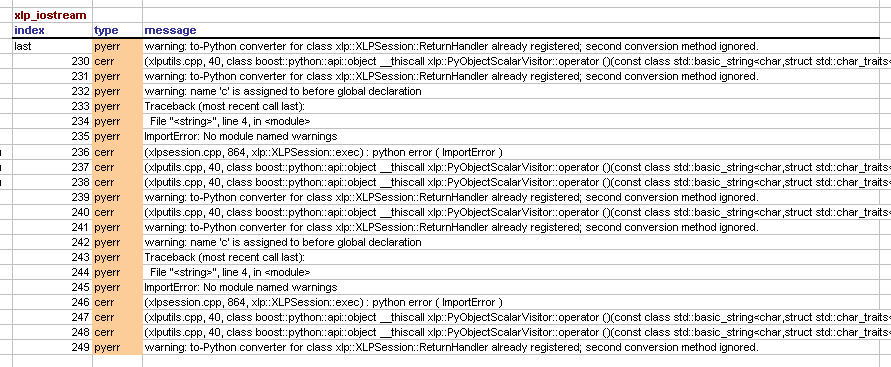
\includegraphics[width=14cm]{images/io.jpg}
\end{xlpfunc}
\end{xlpfunctitle}

\subsection{xlpFullIO}

\begin{xlpfunctitle}{xlpFullIO}

\begin{xlpfunc}{Parameters}
\begin{tabular}{p{3.5cm}cl}
\textbf{trigger}& : & trigger 
\end{tabular}
\end{xlpfunc}


\begin{xlpfunc}{Returns}
A cell matrix of dimension (2048, 3)
\end{xlpfunc}

\begin{xlpfunc}{Description}
\xlp has a circular buffer of 2048 lines storing the standart ouput messages coming from python or c++ (stdout, stderr, std::cout, std::cerr). This function allow to retrieve all the buffer. 

\

The first column represent the message index, the second column the origin of the message (stdout, stderr, std::cout, std::cerr), and the last column store the message itself. 
\end{xlpfunc}
\end{xlpfunctitle}

